\chapter{Estado del Arte\label{sec:estado_del_arte}}

En esta sección se presentan las dos áreas más importantes en las que se ha basado este Trabajo Fin de Grado: el \textit{Computerized Adaptive Testing} o \acrshort{CAT} y la \textit{Adaptive Educational Hypermedia}, o \acrshort{AEH}.

Los \acrshort{CAT} se engloban dentro de una teoría de la psicométrica que exploró por primera vez la posibilidad de hacer exámenes que se adapten de forma automática a las características y el conocimiento del examinado. Primero se detalla la historia, ventajas e inconvenientes que conllevan, además de en qué medida ha influido en este Trabajo. 

A continuación, se detalla las aportaciones de \acrshort{AEH}, una línea de investigación que busca resultados similares al de los \acrshort{CAT} con aportaciones de las investigaciones sobre modelo de usuarios. De nuevo, también se repasa la evolución, ventajas y limitaciones de esta aproximación, además de las aportaciones que ha aportado a este Trabajo.

\section{\textit{Computerized Adaptive Testing}}

A lo largo de toda la historia de la evaluación se ha buscado el equilibrio entre exámenes individuales y colectivos, intentando buscar la evaluación más óptima. En un examen individual se puede lograr una batería de preguntas en las que no haya ninguna inapropiada y asegurar que el evaluado entiende correctamente la tarea. En los exámenes colectivos se asegura que la evaluación ha sido uniforme para todos los evaluados, a la vez que se reducen enormemente el coste de evaluar \cite{Wainer00}.

Durante la década de los setenta aparecieron los primeros trabajos que exploraban la posibilidad de crear exámenes administrados masivamente pero adaptados a los individuos y sus características, eligiendo las nuevas preguntas en función de las respuestas anteriores y ofreciendo una retroalimentación instantánea\cite{Lord68}. Desde un principio fue evidente que este nuevo tipo de evaluación solo sería posible gracias a los ordenadores, por lo que pasó a conocerse como \textit{Computerized Adaptive Testing}.

Entre las mejoras que prometían los \acrshort{CAT} destacaban las siguientes \cite{Green83}:

\begin{enumerate}
	\item \textbf{Aumentan la seguridad de los test}, ya que se almacena un conjunto de preguntas y no solo aquellas preguntas que especificamente se van a realizar. Así, si alguien obtiene acceso a las preguntas no puede mejorar su nota sencillamente estudiando unas cuantas (solo podría mejorar su nota estudiando un porcentaje muy elevado de las preguntas, en cuyo caso se ha ganado esa buena nota).
	\item \textbf{Cada persona puede realizar el examen a su ritmo}, abriendonos a más estilos de respuesta. Además, \texbf{se puede conocer el tiempo que ha tardado en responderse cada pregunta}, información que puede ser útil para evaluar.
	\item \textbf{A todo el mundo se le presenta un reto, sin que nadie se desaliente}. A cada individuo se le presenta las preguntas del rango de dificultad más adecuado para él.
	\item \textbf{Los problemas asociados con el carácter físico de las hojas de respuestras tradicionales desaparecen}. No existe ambigueadad en respuestas a medio marcar o medio borrar, la perdida de la hoja o las dudas sobre lo que está escrito en la hoja.
	\item \textbf{El examen puede ser corregido inmediatamente}, reduciendo el tiempo que el alumno tiene que esperar para obtener retroalimentación, lo cual es especialmente útil en los exámenes dirigidos a ser utilizados para autoevaluación.
	\item \textbf{Facilita realizar un precalibrado de los test}, ya que el sistema puede ir introduciendo discretamente nuevas preguntas para ser calibradas.
	\item \textbf{Se pueden eliminar inmediatamente preguntas defectuosas.}
	\item Una enorme variedad de \textbf{nuevos formatos de preguntas pueden ser explorados}. El sistema de respuesta múltiple no es el único válido. Se pueden crear problemas aritméticas a las que deba introducirse una respuesta numérica. La memoria podría ser evaluada utilizando múltiples marcos. Utilizando sintetizadores de voz, se pueden hacer exámenes de ortografía. Se pueden utilizar vídeos para sustituir largas explicaciones en exámenes de juicio situacional.
\end{enumerate}

Desde entonces, los \acrshort{CAT} se han utilizado con éxito para múltiples propósitos, como la mejora de competencias lingüísticas \cite{Chapelle06} , identificación de estilos de aprendizaje \cite{Ortigosa10}, la habilidad matemática \cite{Klinkenberg11}, o la evaluación del estado de salud \cite{Revicki97}. Así mismo, se ha comprobado que los sistemas educativos que dan retroalimentación inmediata a los alumnos son más efectivos que estrategias de aprendizaje clásicas\cite{Kumar04}. 

A pesar de todas las ventajas que ofrecen, los \acrshort{CAT} han presentado algunos incovenientes que deben ser tratados, aunque múltiples investigaciones han hecho importantes avances. Destacan los siguientes \cite{Wainer00}:

\begin{enumerate}
 	\item \textbf{Nuevos modelos de exámen requieren crear nuevas teorías psicométricas.} Para el caso de los \acrshort{CAT} ha sido bastante utilizada la \textit{Item Response Theory}, o \acrshort{IRT}. La \acrshort{IRT} es un modelo matemático que caracteriza qué ocurre cuando un individuo se encuentra con un pregunta. Cada individuo es caracterizado por un valor de competencia y cada pregunta por una dificultad y se busca elegir la mejor pregunta en función de esos dos valores\cite{Wainer83}.
	\item Los \acrshort{CAT} requieren de una extensa bateria de preguntas, lo que hace compliada \textbf{la correcta calibración de las preguntas}. La estrategia más común para asegurar un buen proceso de calibración implica que la bateria sea provada por una amplia población \cite{Klinkenberg11}. Sin embargo, dado que el pre-calibrado no siempre es posible, se utilizan modelos de estudiantes con el fin de perfeccionar la calidad de la estrategia de evaluación \cite{Antal11}\cite{Galvez09}\cite{Molins14Test}.
	\item En los entornos \acrshort{CAT} hay tres preguntas clave:
	\begin{enumerate}
		\item ¿Cómo se determina con qué pregunta empieza el test?
		\item ¿Cómo se determina la siguiente pregunta que debe plantearse una vez hemos visto la respuesta del examinado a la pregunta actual?
		\item ¿Cómo se determina cuándo parar el test?
	\end{enumerate}
	\textbf{La elección de la respuesta a estas tres preguntas no es trivial ni única.} Existen muchos algoritmos de comienzo, continuación y parada y al ser tres partes claves del flujo que sigue todo \acrshort{CAT} (como se puede ver en la figura \ref{fig:diagrama_flujo_CAT}), la mínima variación en cualquiera de ellos genera sistemas muy distintos. Cada nuevo modelo que aporte un nueva versión de los tres algoritmos necesita ser \textbf{probado para asegurar su confiabiliad, precisión y validez}\cite{Wainer00}.
\end{enumerate}

\begin{figure}[htp!]
	\centering
	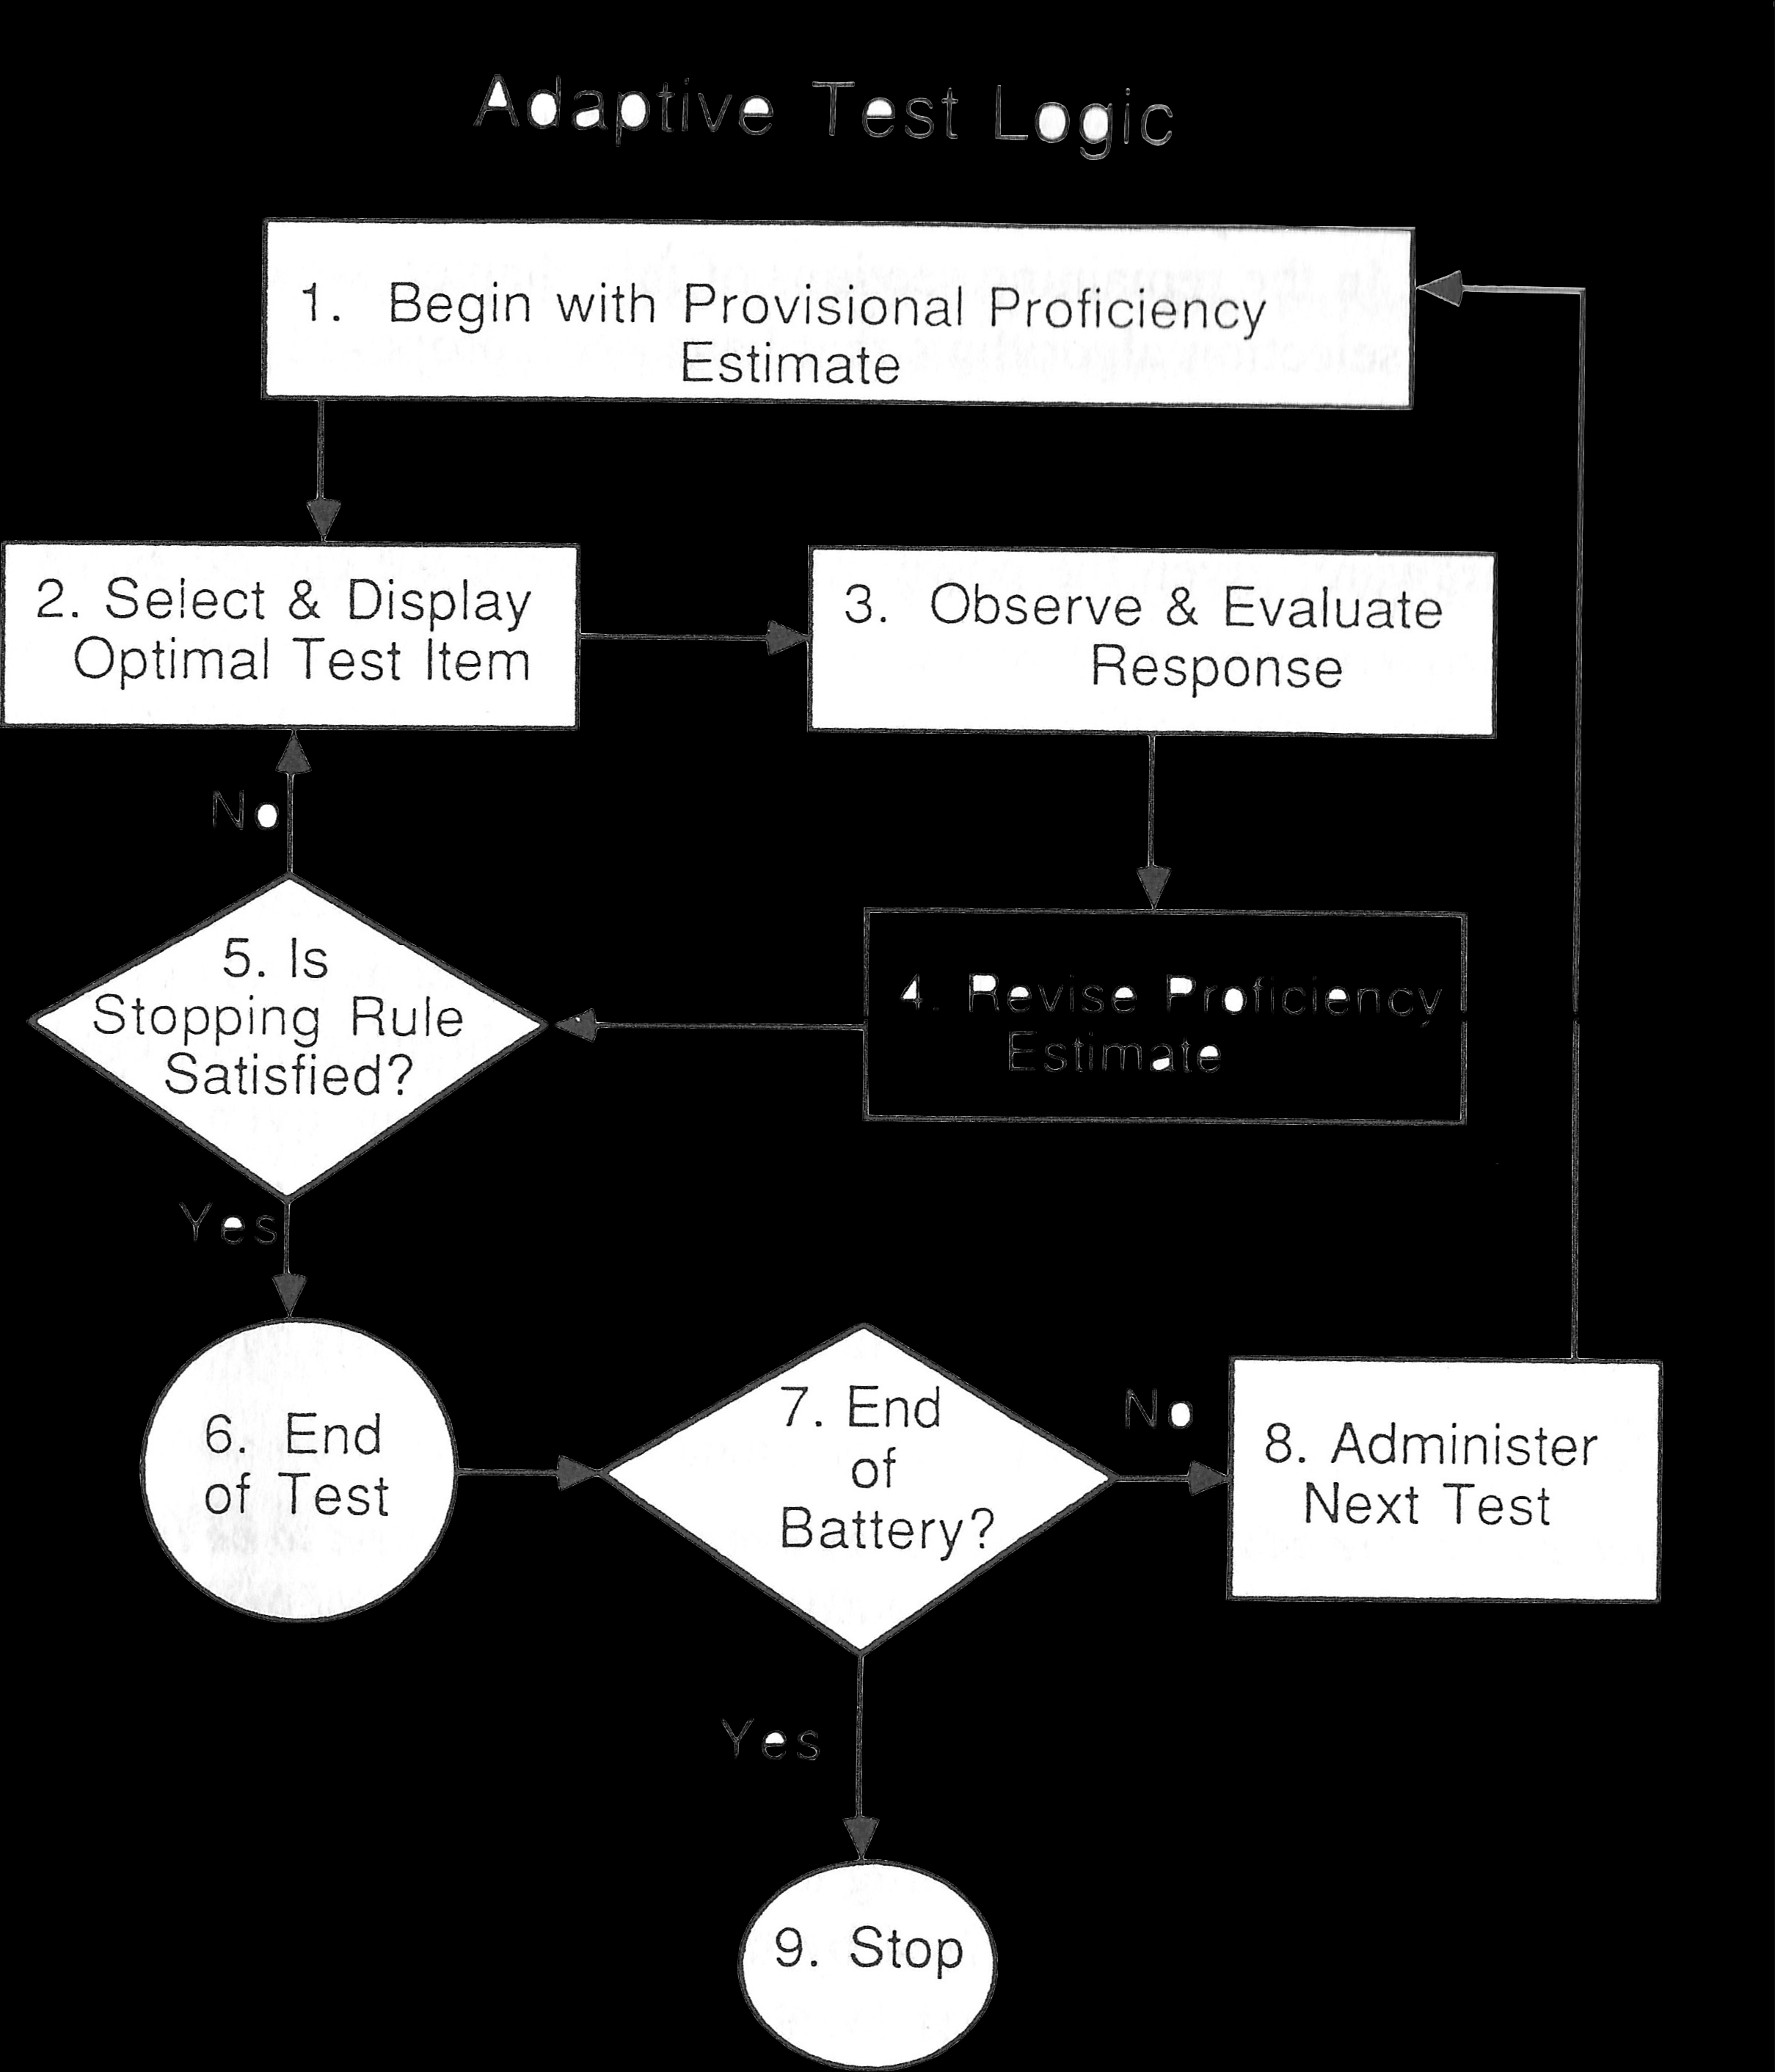
\includegraphics[width=1\textwidth,clip=true]{adaptative_test_logic}
	\caption[Diagrama de flujo de un \acrshort{CAT}]{[Diagrama de flujo de un \acrshort{CAT}]. Diagrama sacado de \cite{Wainer00}}
	\label{fig:diagrama_flujo_CAT}
\end{figure}

El presente TFG toma como punto de partida la teoría sobre los \acrshort{CAT}, aunque con algunas modificaciones. En este Trabajo carece de importancia la parte psicométrica, aunque sí se ha estudiado en la investigación a la que va asociada. Sí que se le ha dado importancia a que el sistema incluya herramientas de anális para cumplir con la promesa de eliminar las preguntas defectuosas, o habilitar posibilidades de nuevos tipos de pregunta, en este caso utilizando ficheros multimedia. El esquema de la figura \ref{fig:diagrama_flujo_CAT} representa una abstracción del flujo que sigue nuestra propuesta, mientras que la elección de la respuesta a las tres preguntas ha venido condicionada por la investigación.
 
\section{\textit{Adaptive Educational Hypermedia}}

Un importante salto ocurrió cuando el la década de los 90 se empezo a investigar la adaptación hipermedia (\acrshort{AH}), y más concretamente, la \textit{adaptive educational hypermedia} o \acrshort{AEH}. \textbf{La madurez de la web presentó una nueva oportunidad} y un desafío para todo tipo de aplicaciones educativas por ordenador. Muchos sistemas adaptativos se movieron a sistemas online, ante las posibilidades que la web ofrecia a estos sistemas\cite{Brusilovsky95}\cite{Nakabayashi97}. Tal fue el interés que para finales de la década todas las tecnologías de la adaptación hipermedia habían sido ya reimplementadas para ser utilizadas sobre la web\cite{Brusilovsky99}.

Desde un principio se detectó que la adaptación era aún más relevante en los sistemas web por, principalmente, dos motivos\cite{Weber01}:

\begin{enumerate}
	\item La mayoría de las aplicaciones educativas basadas en la web tienen en su naturaleza el objetivo de ser \textbf{utilizadas por una variedad mucho más amplia de usuarios} que cualquier aplicación independiente. Una aplicación web diseñada con unos usuarios en mente puede que no se adapte correctamente a otros usuarios.
	\item Los estudiantes suelen trabajar con los sistemas educativos basados en la web por su cuenta (a menudo en casa) y \textbf{no pueden obtener el asistencia inteligente y personalizada que un profesor o la de un estudiante compañero a la que tendría acceso en un aula normal}.
\end{enumerate}

\begin{figure}[htp!]
	\centering
	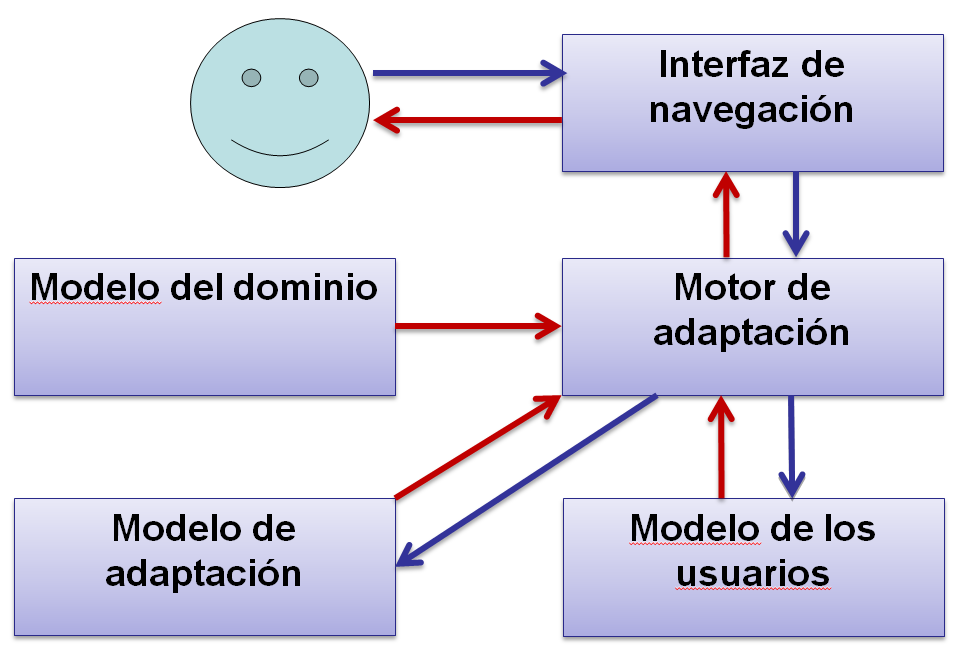
\includegraphics[width=0.75\textwidth,clip=true]{diagrama_disenno}
	\caption{Abstracción de un sistema adaptativo}
	\label{fig:diagrama_disenno}
\end{figure}

Para afrontar el reto de cómo adaptar, \textbf{una abastracción muy utilizada en estos modelos es la de la figura \ref{fig:diagrama_disenno}}\cite{Benyon93}. El usuario (representado arriba a la izquierda) interacciona con el sistema a través de una \textbf{interfaz de navegación} que representa el estado del \textbf{motor de adaptación}, componente que articula al resto de módulos. El modelo del dominio, de adaptación y el modelo de los usuarios son las herramientas de las que el motor de adaptación obtiene la información que le permite dar una respuesta adecuada a cada situación. 

\textbf{El modelo del dominio} recoge las relaciones entre las entidades que componene el dominio del problema. \textbf{El modelo del usuario} a su vez recoge la información que existe sobre el usuario, tanto establecida a priori como observada durante el uso del sistema. \textbf{El modelo de adaptación} recopila la información relativa a cómo debe ir adaptándose la aplicación a los inputs que vaya recibiendo y la información del resto de modelos. Mientras que el modelo del dominio es fijo, en el sentido de que permanece estable durante la vida del mismo, el modelo de adaptación y el modelo de los usuarios van sufriendo variaciones, en función de la entrada que produzcan los usuarios.

En la literatura se distingue entre \textbf{dos conjutnos de técnicas para realizar la adaptación}: la adaptación de contenido y la adaptación de navegación}\cite{Brusilovsky98}. 

\tebf{La adaptación de contenido} tiene como objetivo adaptar la información presentada al usuario de acuerdo a su estilo cognitivo y a sus conocimientos. Para llevar a cabo la adapatación se pueden utilizar las técnicas de texto condicional o la de página condicional. Con la técnica del texto condicional, una página se divide en fragmentos y cada uno es rellando con un texto distinto. Con la técnica de variante de página lo que se hace es tener preparadas varias páginas distintas entre las que se repartirán los usuarios dependiendo de sus características. \textbf{La adaptación de navegación} tiene como objetivo ayudar a los usuarios a encontrar un camino adecuado en un entorno \acrshort{AEG}. Una técnica muy habitual es la manipulación de la selección y la presentación de los enlaces que se muestran al usuario para navegar por la página\cite{Triantafillou03}.

Para la realización de este proyecto, de todas las técnicas englobadas en \acrshort{AEH}, han sido especialmente relevantes la adaptación en módulos expuestos en la figura \ref{fig:diagrama_disenno}, que es la base del diseño de la aplicación, y la adaptación de contenido, que es la técnica que se ha utilizado para realizar la adaptación durante los exámenes que realizan los alumnos.


